\documentclass[10pt]{beamer}
\usepackage{ragged2e} % \justifying
\usepackage[export]{adjustbox} % left and right in images
\usepackage{subcaption} % subfigure
\usepackage[none]{hyphenat} % Avoids to go out of margin
\usetheme{metropolis}           % Use metropolis theme
\title{FP1: Control of the Variable Length Pendulum}
%\subtitle{\textit{Authors:} Xin Xin, Yannian Liu}
\subtitle{Michele Cipriano, Karim Ghonim, Khaled Wahba}
%\date{\today}
\date{}
%\author{Michele Cipriano, Karim Ghonim, Khaled Wahba}
\author{
  \textbf{Control Design and Analysis for Underactuated Robotics:\\
    Variable Length Pendulum}\\
  \textit{Authors:} Xin Xin, Yannian Liu}
\institute{Elective in Robotics: Underactuated Robotics\\
  Department of Computer, Control and Management
  Engineering\\Sapienza University of Rome}

% Fontsize of figure smaller than normalsize:
\setbeamerfont{caption}{size=\scriptsize}

\begin{document}
\nocite{*}

  \maketitle

  \justifying

  \begin{frame}{Introduction}

    \begin{itemize}
      \item the main goal of this work is to study the
        \textbf{Variable Length Pendulum} and present controllers designed
        to make it achieve a desired swing motion 
        given a desired energy and a desired length of the pendulum
      
      \vspace{0.6cm}
      
      \item based on \textbf{Control Design and Analysis for
        Underactuated Robotics: Variable Length Pendulum} by
        \textit{Xin Xin}, \textit{Yannian Liu}

      \vspace{0.6cm}

      \item main points in this work
      \begin{itemize}
        \item motion equation
        \item problem formulation
        \item controller design 
        \item motion analysis
        \item simulation results
      \end{itemize}
    \end{itemize}
  \end{frame}

  \begin{frame}{Motion Equation}
    \begin{columns}[c,onlytextwidth]
      \column{0.6\textwidth}
        \begin{itemize}
          \item friction at pivot $O$ and viscous friction of
            the rod are absent\\
          \item the rod is massless\\
          \item the angle $\theta(t)$ to be between the pendulum and the
            vertical axis\\
          \item the length of the pendulum $l(t)$ starts from the
            origin $O$ to the mass of the pendulum $m$\\
          \item $f(t)$ is the force acting on the mass
        \end{itemize}
      \column{0.4\textwidth}
        \begin{figure}
          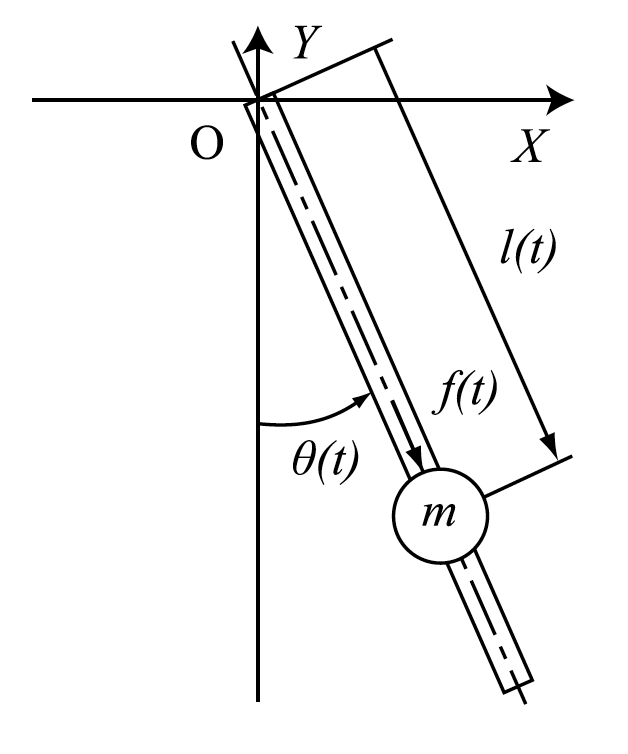
\includegraphics[width=0.96\textwidth,right]{images/vlp.png}
        \end{figure}
    \end{columns}
  \end{frame}

  \begin{frame}{Motion Equation}
    \begin{eqnarray*}
      x_G = l(t)\sin\theta(t) &  y_G = -l(t)\cos\theta(t) 
    \end{eqnarray*}
    kinetic energy defined as
    \begin{equation*}
      T = \frac{1}{2}m(\dot{x}_G^2+\dot{y}_G^2) = \frac{1}{2}m\big(l(t)\dot{\theta}(t)\big)^2+\frac{1}{2}m\big(\dot{l}(t)\big)^2 
    \end{equation*}
    potential energy as
    \begin{equation*}
      P = mgy_G = -mgl(t)\cos\theta(t)  
    \end{equation*}
    the Lagrangian equation of the VLP
    \begin{equation*}
      L = T-P
    \end{equation*}
    Euler-Lagrangian operator 
    \begin{equation*}\label{model}
      \frac{\partial L}{\partial q}   -\frac{dL}{dt}\Bigg(\frac{\partial L}{\partial \dot{q}}\Bigg) = \tau
    \end{equation*}
  with $q = [l, \theta]^T$ and $\tau$ applied generalized forces
  \end{frame}

  \begin{frame}{Motion Equation}
    Euler-Lagrange equation
    \begin{align*}
      &\ddot{\theta}(t)+\frac{2\dot{l}(t)\dot{\theta}(t)}{l(t)}+
        \frac{g\sin\theta(t)}{l(t)} = 0  \\
      &\ddot{l}(t)-ml(t)\dot{\theta}^2(t)-mg\cos\theta(t) = f(t)
    \end{align*}
    control input
    \begin{equation*}
      u = \ddot{l}(t)
    \end{equation*}
  \end{frame}

  \begin{frame}{Problem Formulation}
    let $m=1$, total mechanical energy
    \begin{equation*}
      E_T = %T+P =
        \frac{1}{2}\dot{l}^2(t)+\frac{1}{2}\big(l(t)\dot{\theta}(t)\big)^2-
        gl(t)\cos\theta(t) 
    \end{equation*}
    desired trajectory of swing described by
    \begin{equation*}
      E_r = \frac{1}{2}\big(l_r\dot{\theta}(t)\big)^2-gl_r\cos\theta(t) 
    \end{equation*}
    with $E_r$ and $l_r$ desired energy and length of the VLP
    \\
    $E_r = -gl_r\cos\theta_{max}, \theta_{max} \in (0,\pi]$

    \textbf{Trajectory tracking control problem}
    \begin{equation*}
      \lim_{t\rightarrow \infty} E_T = E_r  \quad
      \lim_{t\rightarrow \infty} \dot{l} = 0 \quad
      \lim_{t\rightarrow \infty} l = l_r
    \end{equation*}
  \end{frame}

  \begin{frame}{Controller Design: Total Energy Shaping}
    Lyapunov candidate with $k_P>0$, $k_D>0$
    \begin{gather*}
      V_c = \frac{1}{2}(E_T-E_r)^2+\frac{1}{2}k_P(l-l_r)^2+
        \frac{1}{2}k_D\dot{l}^2 \\
      \dot{V}_c = \dot{l}\big((E_T-E_r+k_D)u-(E_T-E_r)(l\dot{\theta}^2+
        g\cos\theta)-k_P(l-l_r) \big)
    \end{gather*}
    controller
    \begin{equation*}
      u = \frac{(E_T-E_r)(l\dot{\theta}^2+g\cos\theta)-k_P(l-l_r)-
        k_V\dot{l}}{E_T-E_r+k_D}
    \end{equation*}
    with $k_V>0$, then
    \begin{equation*}
      \dot{V}_c = -k_V\dot{l}^2 \leq 0
    \end{equation*}
    which holds only if
    \begin{equation*}
      E_T-E_r+k_D  \neq 0 \quad \forall t\geq 0
    \end{equation*}
  \end{frame}

  \begin{frame}{Total Energy Shaping: Simulation}
    consider the trajectory tracking control problem defined previously
    and $l_r=3\text{m}$, $\theta_{\max}=2\pi/5$, $g=9.81\text{m/s}^2$
    
    \vspace{1cm}
    
    let $k_D=12$, $k_P=30$ and $k_V=12$
  \end{frame}

  \begin{frame}{Total Energy Shaping: Simulation}
    \begin{figure}
      \caption*{Time responses of $V$, $E_T-E_r$, $E_T-E_r+k_D$ and $u$
        with initial state
        $(\theta(0),l(0),\dot{\theta}(0),\dot{l}(0)) = (-\pi/6,2,0,0)$}
      \vspace{-0.3cm}
      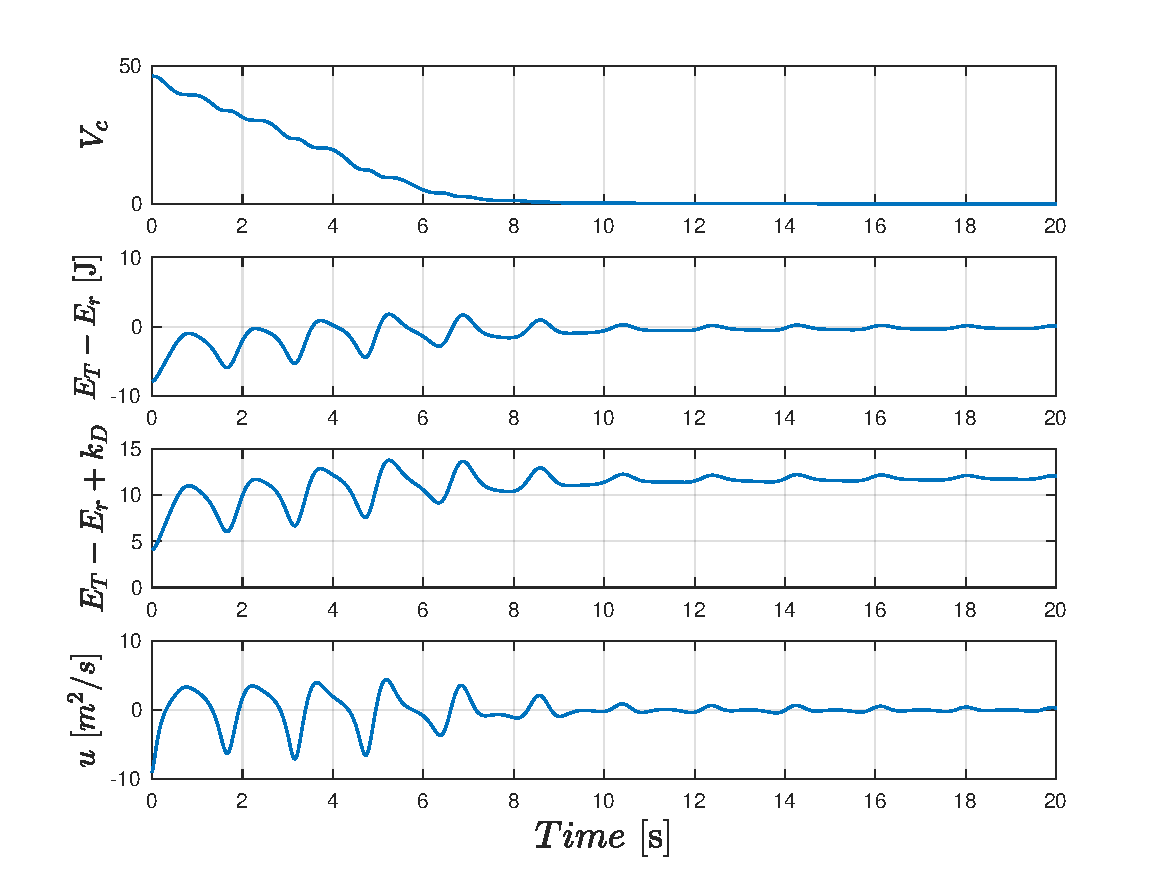
\includegraphics[width=0.8\textwidth]{images/total_1b.pdf}
    \end{figure}
  \end{frame}

  \begin{frame}{Total Energy Shaping: Simulation}
    \begin{figure}
      \caption*{Time reponses of $(\theta,l,\dot{\theta},\dot{l})$ with initial
        state $(\theta(0),l(0),\dot{\theta}(0),\dot{l}(0))=(-\pi/6,2,0,0)$}
      \vspace{-0.3cm}
      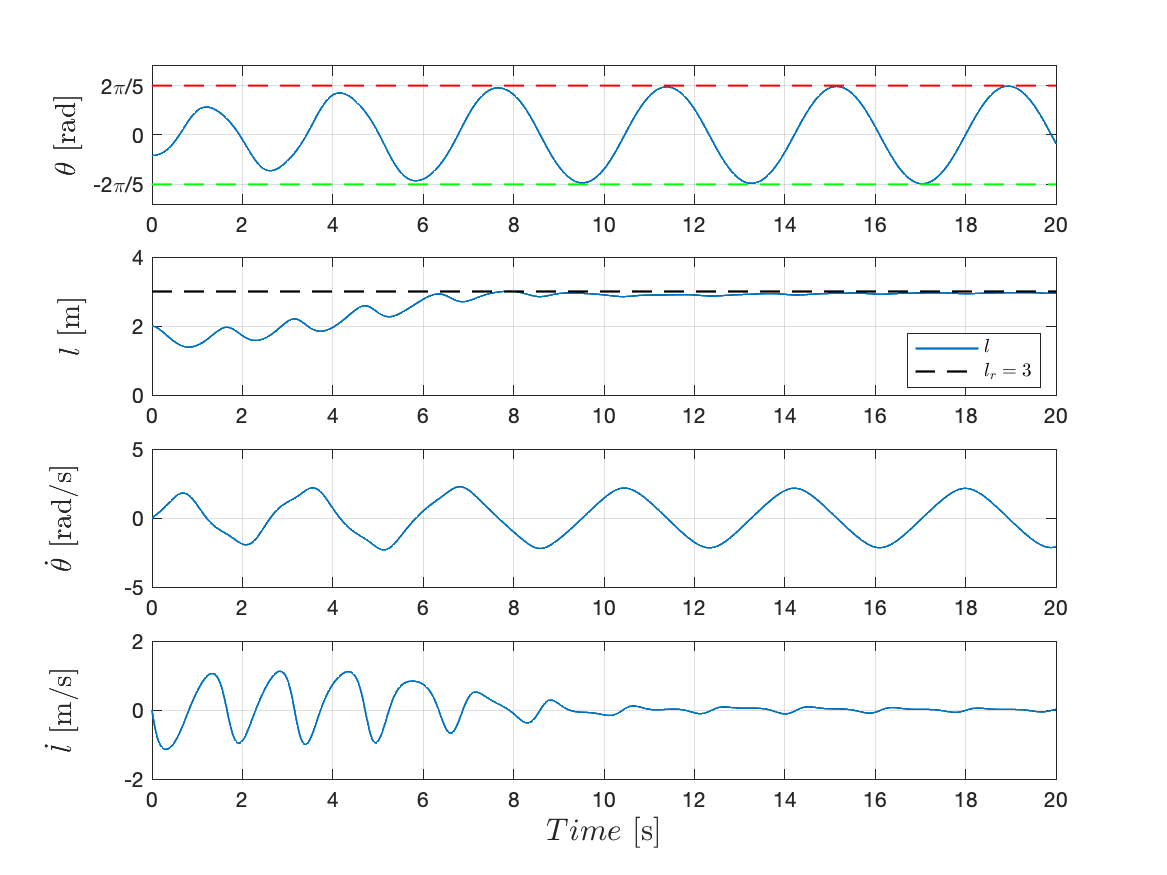
\includegraphics[width=0.8\textwidth]{images/total_2b.pdf}
    \end{figure}
  \end{frame}

  \begin{frame}{Total Energy Shaping: Simulation}
    \begin{figure}
      \caption*{The controller encountered a
        singular point for initial state $(\theta(0),l(0),\dot{\theta}(0),
        \dot{l}(0)) = (-\pi/6,2,0,4)$}
      \vspace{-0.3cm}
      \begin{subfigure}{.49\textwidth}
        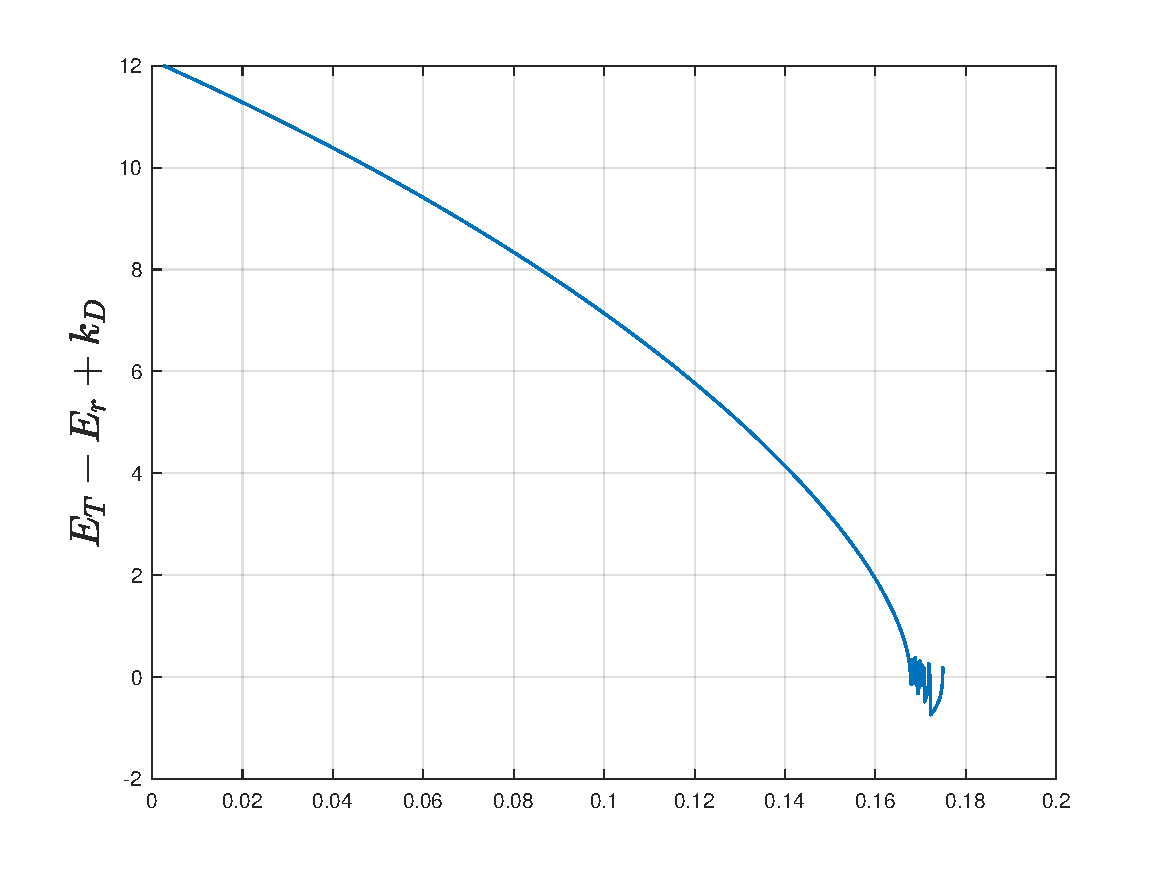
\includegraphics[width=1\linewidth]{images/total_2.pdf}
      \end{subfigure}
      \begin{subfigure}{.49\textwidth}
        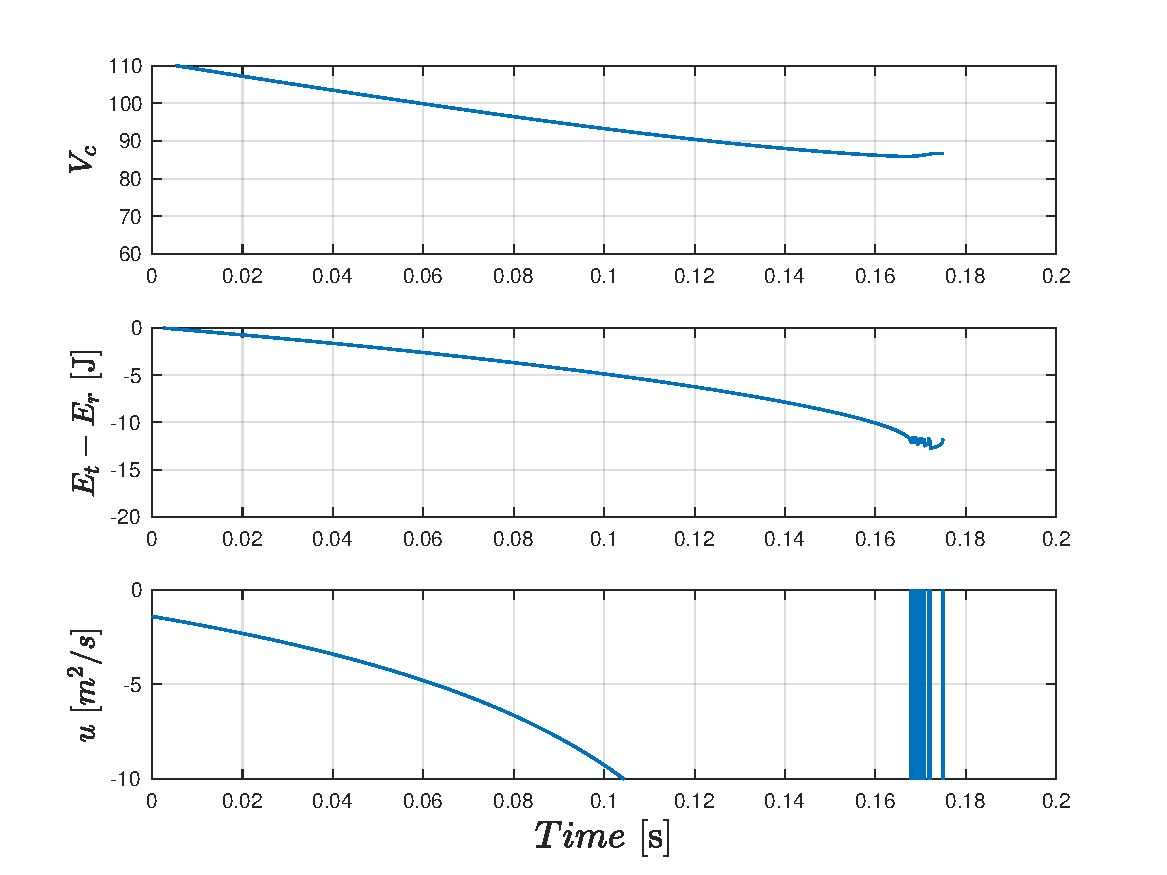
\includegraphics[width=1\linewidth]{images/total_1.pdf}
      \end{subfigure}  
    \end{figure}
  \end{frame}
  
  \begin{frame}{Controller Design: Partial Energy Shaping}
    $E_P$ sum of kinetic energy of rotation and potential energy of VLP
    \begin{equation*}
      E_P = \frac{1}{2}(l(t)\dot{\theta}(t))^2-gl(t)\cos\theta(t)
    \end{equation*}
    since $(E_T, l, \dot{l}) \equiv (E_r, l_r, 0)$ equivalent to
    $(E_P, l, \dot{l}) \equiv (E_r, l_r, 0)$
    \\
    Lyapunov candidate
    \begin{gather*}
      V = \frac{1}{2}(E_P-E_r)^2+\frac{1}{2}k_P(l-l_r)^2+
        \frac{1}{2}k_D\dot{l}^2 \\ 
      \dot{V} = \big(-(E_P-E_r)(l\dot{\theta}^2+g\cos\theta)+k_P(l-l_r)\big)
        + k_D u) \dot{l}
    \end{gather*}
    controller
    \begin{equation*}
      u = \frac{(E_P-E_r)(l\dot{\theta}^2+g\cos\theta)-k_P(l-l_r)
        -k_V\dot{l}}{k_D}
    \end{equation*}
    which is free of singular points
    \begin{equation*}
      \dot{V} = -k_V \dot{l}^2 \le 0, \quad k_V > 0
    \end{equation*}
  \end{frame}

  \begin{frame}{Controller Design: Partial Energy Shaping}
    consider
    \begin{equation*}
      \Gamma_c = \left\{(\theta,l,\dot{\theta},\dot{l})|
        V(\theta,l,\dot{\theta},\dot{l}) \le c\right\}, \quad c > 0
    \end{equation*}
    since $\dot{V} \le 0$, any closed-loop solution starting in $\Gamma_c$
    remains in $\Gamma_c$ for all $t \ge 0$
    
    let $W$ be the largest invariant set in
    \begin{equation*}
      S = \{(\theta,l,\dot{\theta},\dot{l}) \in \Gamma_c|\dot{V}=0\}
    \end{equation*}
    using \textbf{LaSalle's invariant principle}, every closed-loop
    solution starting in $\Gamma_c$ approaches $W$ as $t \to \infty$
  \end{frame}

  \begin{frame}{Controller Design: Partial Energy Shaping}
    since $\dot{V} = 0$ holds for all elements of $W$, then
    \begin{equation*}
      V \equiv V^* \quad l \equiv l^*
    \end{equation*} 
    moreover,
    since $V$ is a constant in $W$, $E_P$ is also a constant in $W$
    \begin{equation*}
      \lim_{t\rightarrow \infty} E_P = E^* \quad
      \lim_{t\rightarrow \infty} \dot{l} = 0 \quad
      \lim_{t\rightarrow \infty} l = l^*
    \end{equation*}     
    thus, the largest invariant set $W$ can be defined as
    \begin{equation*}
      W = \left\{(\theta,l,\dot{\theta},\dot{l})\middle|
        \frac{1}{2}(l^*\dot{\theta})^2-gl^*\cos\theta \equiv E^*,
        l \equiv l^*\right\}
    \end{equation*}
  \end{frame}

  \begin{frame}{Motion Analysis: Convergence of Energy}
    Trajectory Tracking Control Problem achieved iff $V^*=0$, with
    \begin{equation*}
      V^* = \frac{1}{2}(E^*-E_r)^2+\frac{1}{2}k_P(l^*-l_r)^2
    \end{equation*}
    consider $E_P \equiv E^*$, $l \equiv l^*$, $\dot{l} \equiv 0$
    and $u = \ddot{l} \equiv 0$, then, from the controller
    based on partial energy shaping
    \begin{equation*}
      (E^*-E_r)(l^*\dot{\theta}^2+g\cos\theta)-k_P(l^*-l_r) \equiv 0
    \end{equation*}
  \end{frame}

  \begin{frame}{Motion Analysis: Convergence of Energy}
    \noindent \textbf{Case 1:} $E^* = E_r$

    $l^* = l_r$, the largest invariant set $W$ becomes
    \begin{equation*}
      W_r = \left\{ (\theta, l, \dot{\theta}, \dot{l})
        \middle| \frac{1}{2} (l_r \dot{\theta})^2 -
        g l_r \cos\theta \equiv E_r, l \equiv l_r \right\}
    \end{equation*}
    hence, as $t \to \infty$, the closed-loop solution
    $(\theta(t), l(t), \dot{\theta}(t), \dot{l}(t))$ achieves the
    tracking control objective
  \end{frame}

  \begin{frame}{Motion Analysis: Convergence of Energy}
    \noindent \textbf{Case 2} $E^* \neq E_r$
    \begin{equation*}
      l^* \dot{\theta}^2 + g\cos\theta \equiv \frac{k_P(l^*-l_r)}{E^*-E_r}
    \end{equation*}
    since $E_P \equiv E^*$, $l \equiv l^*$, from the definition of $E_P$
    \begin{equation*}
      l^* \dot{\theta}^2 - 2g\cos\theta \equiv \frac{2E^*}{l^*}
    \end{equation*}
    taking the difference between the two shows
    that $\theta$ is a constant
    \begin{equation*}
      \theta \equiv \theta^*
    \end{equation*} 
    since $E_r = -g l_r \cos\theta_{\max}$
    \begin{equation*}
      l^* = \frac{l_r(k_P+g^2\cos\theta_{\max}\cos\theta^*)}{k_P+g^2}
    \end{equation*}
  \end{frame}

  \begin{frame}{Motion Analysis: Convergence of Energy}
    from the dynamics of the VLP $\sin\theta^*=0$, which admits a solution
    only in
    $\{0, \pi\}$, hence, either $(\theta^*, l^*)=(\pi, l_{ue})$ or $(\theta^*,
    l^*)=(0, l_{de})$ where
    \begin{align*}
      l_{ue} = l^*\rvert_{\theta^*=\pi} &=
        \frac{l_r(k_P-g^2\cos\theta_{\max})}{k_P+g^2} \\
        l_{de} = l^*\rvert_{\theta^*=0} &=
        \frac{l_r(k_P+g^2\cos\theta_{\max})}{k_P+g^2}
    \end{align*}
    to guarantee that $l_{ue}, l_{de} > 0$ assume
    \begin{equation*}
      k_P > g^2 |\cos\theta_{\max}|
    \end{equation*}
  \end{frame}

  \begin{frame}{Motion Analysis: Convergence of Energy}
    considering also that $0 < \theta_{\max} \le \pi$,
    it is easy to prove that
    \begin{gather*}
        0 < l_{ue} \le l_r \\ 0 < l_{de} < l_r
    \end{gather*}
    let $\Omega$ be the equilibrium point set (invariant set) defined as
    \begin{equation*}
      \Omega = \{ (\pi, l_{ue}, 0, 0), (0, l_{de}, 0, 0) \}
    \end{equation*}
  \end{frame}

  \begin{frame}{Motion Analysis: Closed-Loop Equilibrium Points}
    let the state variable vector be $x = (\theta, l, \dot{\theta},
    \dot{l})^T$, considering the dynamics of the VLP and the controller based
    on partial energy shaping, the state space representation is 
    \begin{align*}
      \dot{x}_1 &= x_3 \\
      \dot{x}_2 &= x_4 \\
      \dot{x}_3 &= -\frac{2 x_3 x_4 + g\sin x_1}{x_2} \\
      \dot{x}_4 &= \frac{(E_P-E_r)(x_2 x_3^2 + g\cos x1)
        -k_P(x_2-l_r)-k_V x_4}{k_D}
    \end{align*}
    where $E_P=x_2^2 x_3^2 / 2 - g x_2 \cos x_1$
  \end{frame}

  \begin{frame}{Motion Analysis: Closed-Loop Equilibrium Points}
    characteristic equation of the Jacobian evaluated
    at $x_{ue} = (\pi, l_{ue}, 0, 0)^T$
    \begin{equation*}
      det(sI-A_{ue}) = \left( s^2 + \frac{k_V}{k_D}s +
        \frac{g^2+k_P}{k_D} \right) \left( s^2 - \frac{g}{l_{ue}}\right)
    \end{equation*}
    $A_{ue}$ has three eigenvalues in open LHP and
    one in open RHP
    
    $x_{ue}$ is \textbf{unstable} and \textbf{hyperbolic}
  \end{frame}

  \begin{frame}{Motion Analysis: Closed-Loop Equilibrium Points}
    characteristic equation of the Jacobian evaluated
    at $x_{de} = (0, l_{de}, 0, 0)^T$
    \begin{equation*}
      det(sI-A_{de}) = \left( s^2 + \frac{k_V}{k_D}s +
        \frac{g^2+k_P}{k_D} \right) \left( s^2 + \frac{g}{l_{ue}}\right)
    \end{equation*}
    $A_{de}$ has two eigenvalues in open LHP and two on imaginary axis
    
    $x_{de}$ is \textbf{non-hyperbolic}
  \end{frame}

  \begin{frame}{Motion Analysis: Closed-Loop Equilibrium Points}
    consider the Lyapunov function V used for partial energy shaping
    \begin{equation*}
      V = \frac{1}{2}(E_P-E_r)^2+\frac{1}{2}k_P(l-l_r)^2+
        \frac{1}{2}k_D\dot{l}^2
    \end{equation*}
    consider the following set
    \begin{equation*}
      \Gamma_d = \left\{ (\theta, l, \dot{\theta}, \dot{l})
        \mid V(\theta, l, \dot{\theta}, \dot{l}) <
        V(0, l_{de}, 0, 0) \right\}
    \end{equation*}
    let the values of V at $x_{de}$
    and at $(\delta, l_{de}, 0, 0)$ respectively be
    \begin{gather*}
      V_{de} = V(0, l_{de}, 0, 0) = \frac{1}{2}(g l_{de} + E_r)^2
        + \frac{1}{2} k_P (l_{de} - l_r)^2 \\
      V_\delta = V(\delta, l_{de}, 0, 0) = \frac{1}{2}(g l_{de}
        \cos\delta + E_r)^2 + \frac{1}{2} k_P (l_{de} - l_r)^2
    \end{gather*}
  \end{frame}

  \begin{frame}{Motion Analysis: Closed-Loop Equilibrium Points}
    \begin{align*}
      V_\delta - V_{de} %&= -\frac{1}{2} g l_{de} (1-\cos\delta)
        %(g l_{de}(1+\cos\delta)+2E_r) \\
        &= -\frac{g^2 l_{de} l_r (1-\cos\delta) \Xi}{k_P+g^2}
    \end{align*}
    \begin{equation*}
        \Xi = k_P(1-\cos\theta_{\max})-(k_P+g^2\cos\theta_{\max})
            \sin^2 \left( \frac{\delta}{2} \right)
    \end{equation*}
    using $k_P > -g^2\cos\theta_{\max}$ and
    $|\sin \delta|<|\delta|$ for $\delta \neq 0$
    \begin{equation*}
      \Xi > k_P(1-\cos\theta_{\max})-
        \frac{(k_P+g^2\cos\theta_{\max})\delta^2}{4}
    \end{equation*}
    with $\delta \neq 0$
  \end{frame}

  \begin{frame}{Motion Analysis: Closed-Loop Equilibrium Points}
    if $\delta$ satisfies
    \begin{equation*}
      0 < |\delta| \le \delta_m = 2
        \sqrt{\frac{k_P(1-\cos\theta_{\max})}{k_P+g^2\cos\theta_{\max}}}
    \end{equation*}
    then $\Xi>0$,
    which, using $V_\delta - V_{de}$, implies
    \begin{equation*}
      V_\delta < V_{de}, \quad (\delta, l_{de}, 0, 0) \in \Gamma_d
    \end{equation*}
    which itself implies%, because of the definition of $\Gamma_d$,
    that $\Gamma_d \neq \varnothing$

    $x_{de}$ is \textbf{unstable} in the Lyapunov sense
  \end{frame}

  \begin{frame}{Motion Analysis: Closed-Loop Equilibrium Points}
    every closed-loop solution under the closed-loop
    system consisted of the dynamic equation of the VLP and the controller
    based on partial energy shaping, supposing
    \begin{gather*}
    0<\theta_{\max}\le\pi \\
    k_P>g^2|\cos\theta_{\max}|, \quad k_D>0, \quad k_V>0
    \end{gather*}
    approaches $W=W_r\cup\Omega$
  \end{frame}

  \begin{frame}{Partial Energy Shaping: Simulation}
    consider the trajectory tracking control problem defined previously
    and $l_r=3\text{m}$, $\theta_{\max}=2\pi/5$, $g=9.81\text{m/s}^2$
    
    the condition on $k_P$ is 
    \begin{equation*}
      k_P > g^2 |cos\theta_{\max}| = 29.74
    \end{equation*}
    which yields $l_{de}=1.42$m

    \vspace{1cm}
    
    let $k_D=12$, $k_P=30$ and $k_V=12$
  \end{frame}

  \begin{frame}{Partial Energy Shaping: Simulation}
    \begin{figure}
      \caption*{Time responses of $V$, $E_P-E_r$ and $u$ with initial state 
        $(\theta(0), l(0), \dot{\theta}(0), \dot{l}(0))=(-\pi/6, 2, 0, 0)$}
      \vspace{-0.3cm}
      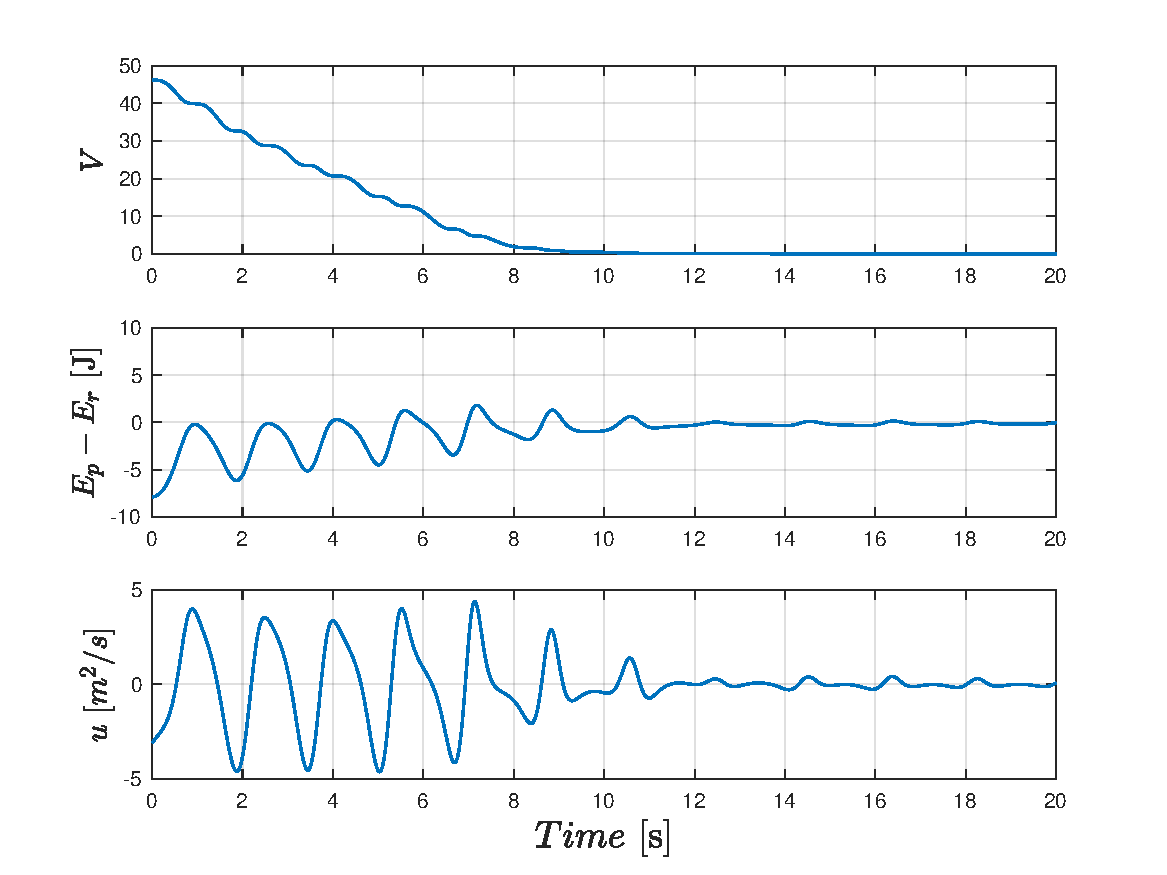
\includegraphics[width=0.8\textwidth]{images/partial_1.pdf}
    \end{figure}
  \end{frame}

  \begin{frame}{Partial Energy Shaping: Simulation}
    \begin{figure}
      \caption*{Time responses of $(\theta, l, \dot{\theta}, \dot{l})$ with 
        initial state $(\theta(0), l(0), \dot{\theta}(0), \dot{l}(0))=
        (-\pi/6, 2, 0, 0)$}
      \vspace{-0.3cm}
      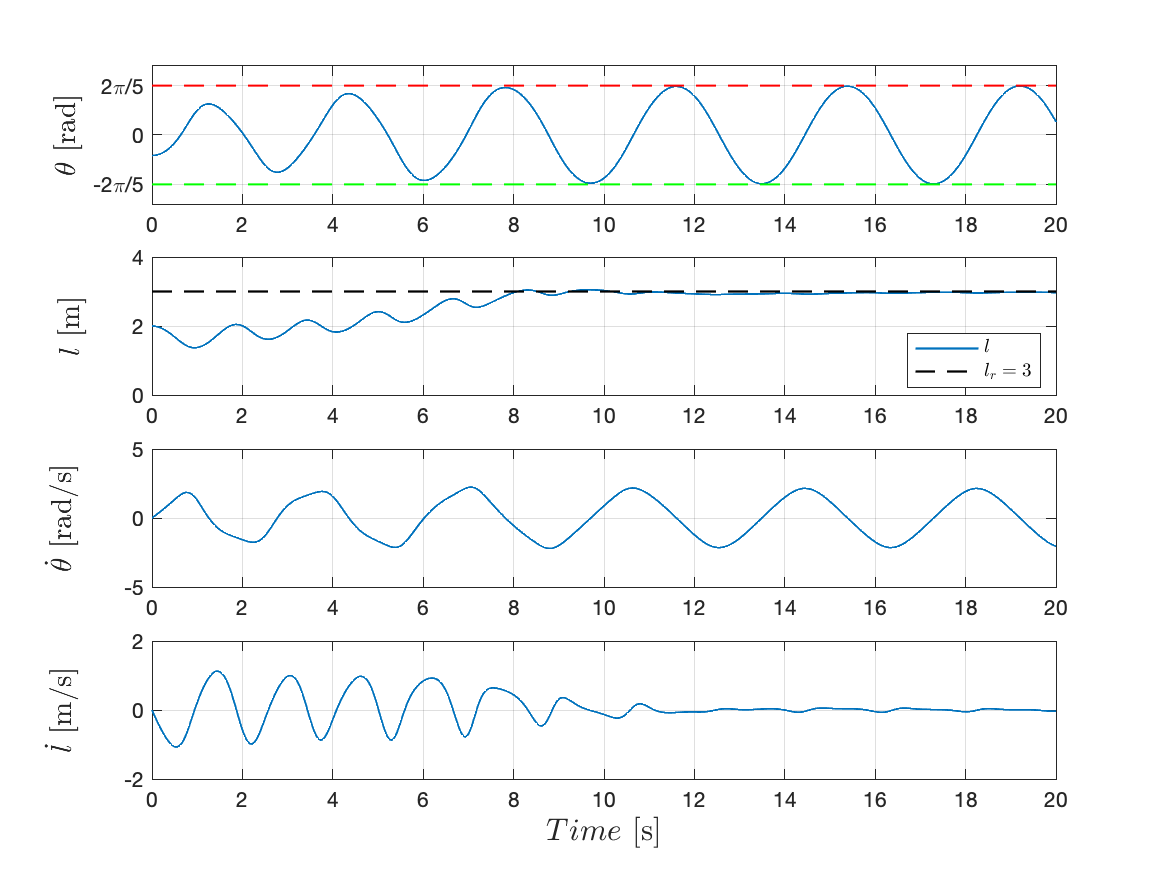
\includegraphics[width=0.8\textwidth]{images/partial_2.pdf}
    \end{figure}
  \end{frame}

  \begin{frame}{Partial Energy Shaping: Simulation}
    \begin{figure}
      \caption*{Time responses of $V$, $E_P-E_r$ and $u$ with initial state 
        $(\theta(0), l(0), \dot{\theta}(0), \dot{l}(0))=(-\pi/3, l_{de}, 0,
        0)$, which satisfied $V_\delta < V_{de}$}
      \vspace{-0.3cm}
      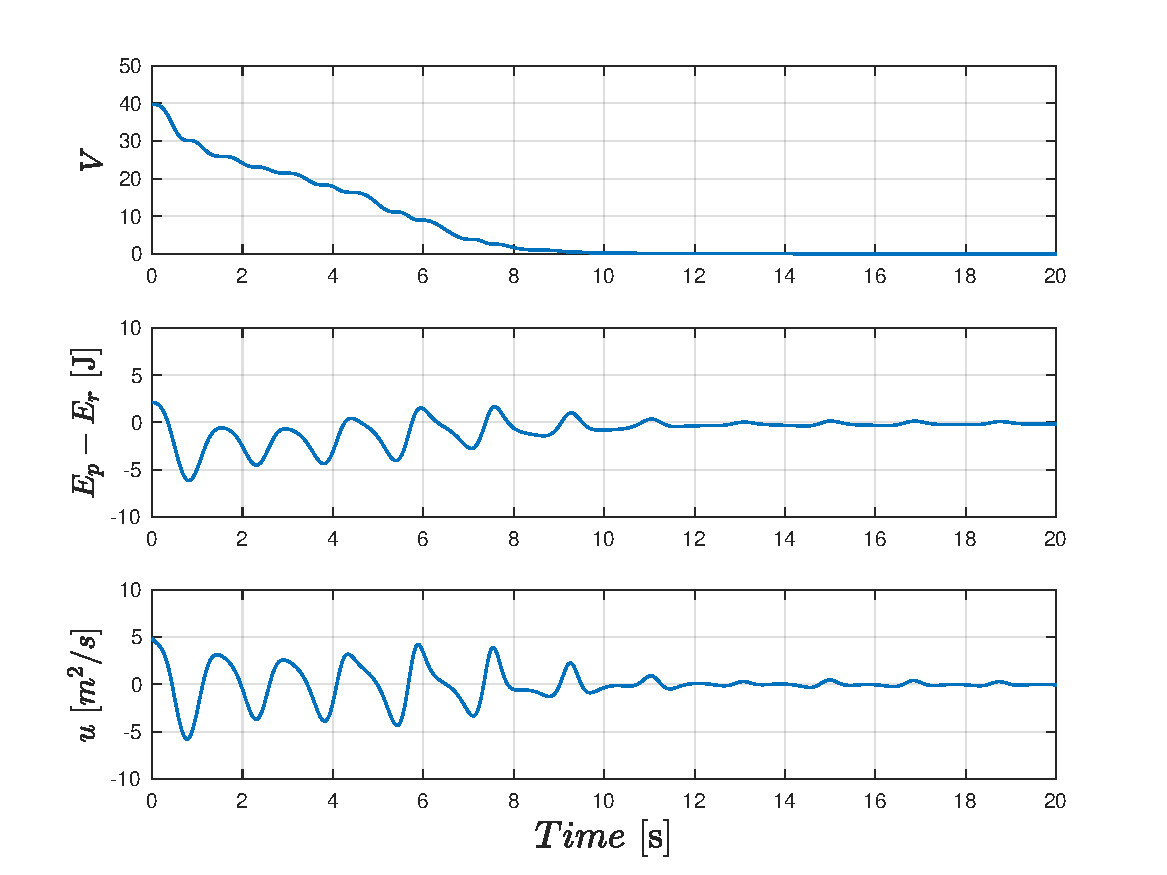
\includegraphics[width=0.8\textwidth]{images/partial_1b.pdf}
    \end{figure}
  \end{frame}

 \begin{frame}{Partial Energy Shaping: Simulation}
    \begin{figure}
      \caption*{Time responses of $(\theta, l, \dot{\theta}, \dot{l})$ with 
        initial state $(-\pi/3, l_{de}, 0, 0)$}
      \vspace{-0.3cm}
      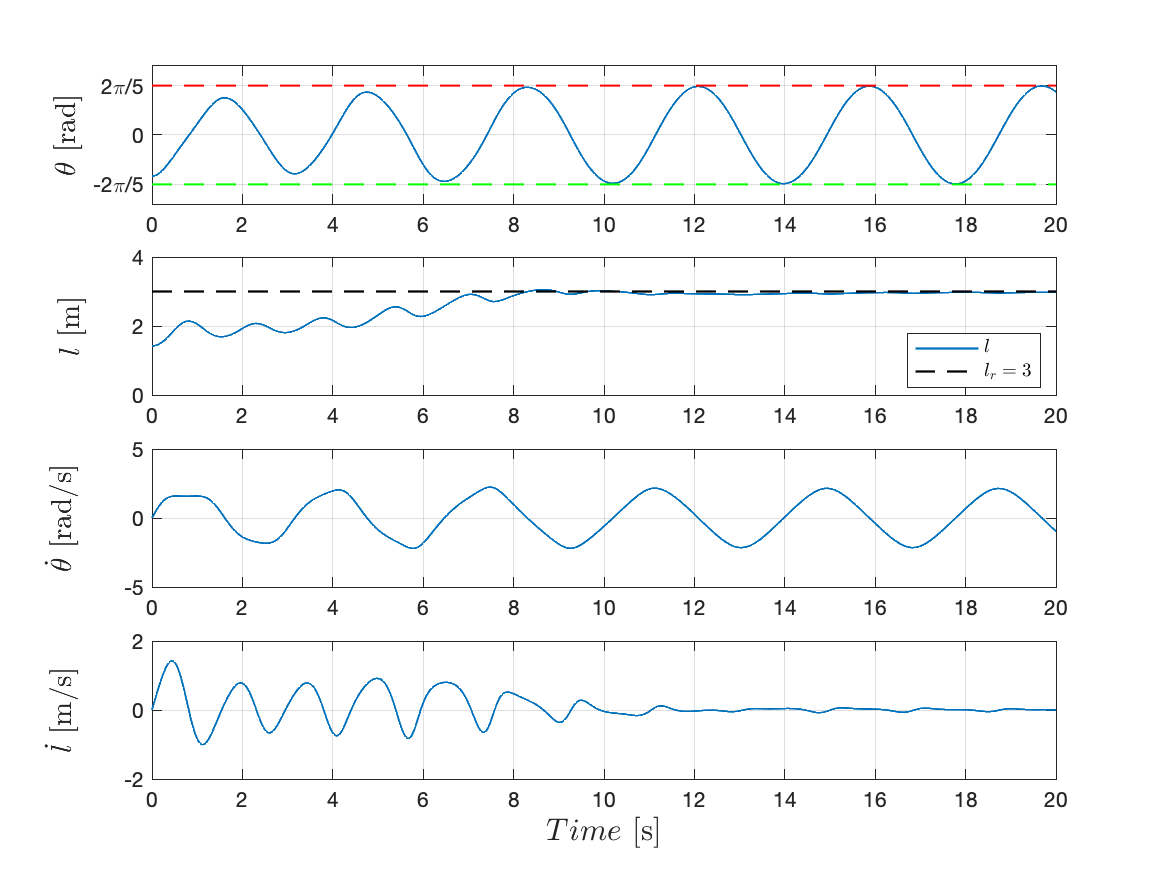
\includegraphics[width=0.8\textwidth]{images/partial_2b.pdf}
    \end{figure}
  \end{frame}

\begin{frame}[standout]
    Q\&A
  \end{frame}

  \appendix

  \begin{frame}{References}
    \bibliography{bibliography}
    \bibliographystyle{ieeetr}
  \end{frame}

\end{document}
